In this section, we present single-core benchmarks for the components of our implementation followed by parallel decompression benchmarks.
All benchmarks in this section were executed on a single exclusively allocated \anon[cluster node]{AMD Rome cluster node provided by the Technische Universität Dresden}.
Each cluster node contains \SI{512}{\gibi\byte} of main memory and \num{2} AMD EPYC CPU 7702 processors with \num{64} cores each and with enabled simultaneous multithreading.
This yields a total of \num{256} virtual cores with a base clock frequency of \SI{2}{\giga\hertz}.

\subsection{Bit Reader}

\begin{figure}
    \centering
    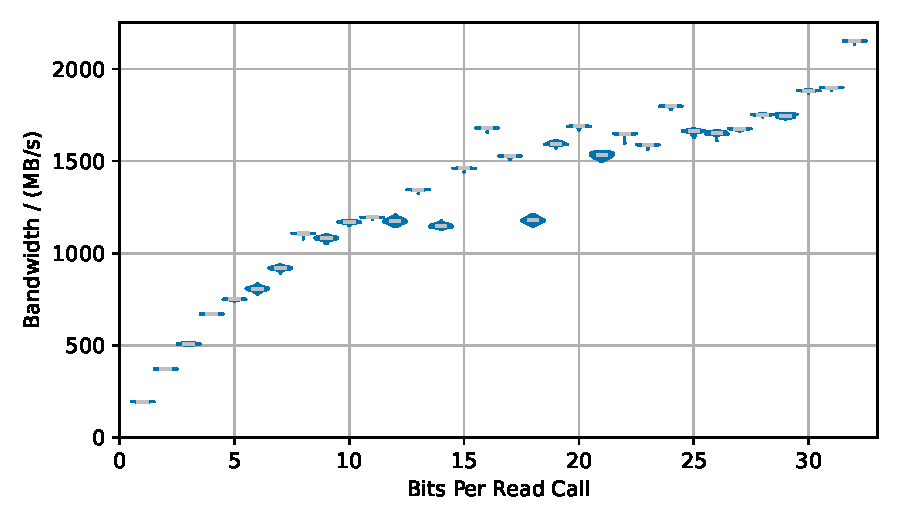
\includegraphics[width=\linewidth]{plots/bitreader-bandwidths-over-bits-per-read.pdf}
    \caption{
        The \texttt{BitReader::read} method has been called with the given number of bits in a loop until the end of the data has been reached.
        The benchmark is single-threaded.
        The violin plot displays the sampled results from repeating the benchmarks 100 times.
        The data used for testing measures \SI{2}{\mebi\byte} scaled by the bits-per-read to give approximately equal benchmark runtimes.
    }
    \label{fig:bitreader}
\end{figure}

\Cref{fig:bitreader} shows that the performance of the \texttt{BitReader} class increases with the number of requested bits per call.
Thus, the bit reader should be queried as rarely as possible with as many bits as possible for optimal performance.
The number of requested bits depends on the Huffman decoder and the \blockfinder implementation.
One of the implemented Huffman decoders always requests the maximum \huffcode length, which is 15 bits for \deflate.

The parallelized gzip decompressor uses separate \texttt{BitReader} instances in each thread.
This increases the aggregated bit reader bandwidth accordingly.
Comparing the compressed bandwidth in \cref{fig:bitreader} and the decompressed bandwidth in \cref{fig:parallel-decompression} shows that the bit reader is not the main bottleneck even for the worst case with a compression ratio of 1.


\subsection{File Reader}

\begin{figure}
    \centering
    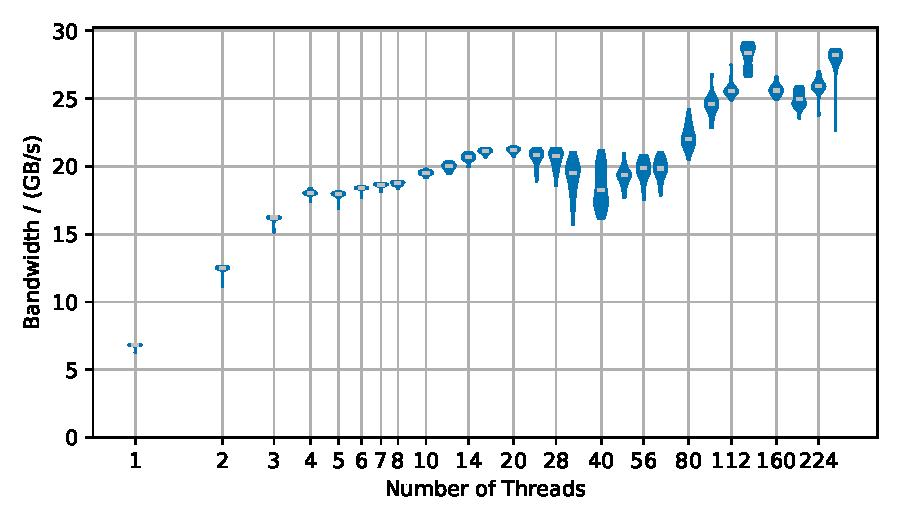
\includegraphics[width=\linewidth]{plots/filereader-bandwidths-number-of-threads-sequential-pinning.pdf}
    \caption{
        The \texttt{SharedFileReader} class is used from a set number of threads to read the file contents of a \SI{1}{\gibi\byte} large file located in \texttt{/dev/shm} in a strided manner.
        The implementation uses POSIX pread to read in parallel from the file.
        Each thread reads a \SI{128}{\kibi\byte} chunk, skips over the subsequent chunks read by other threads, and then reads the next chunk.
        The violin plot displays the sampled results from repeating the benchmarks 100 times.
    }
    \label{fig:filereader}
\end{figure}

\Cref{fig:filereader} shows results for multiple threads reading the same file residing in the in-memory file system \texttt{/dev/shm} in parallel.
The file was created by the main thread that has been pinned to core 0.
The n-th reader thread is pinned to the n-th core.
Each NUMA domain spans 16 physical cores.
The first NUMA domain consists of cores 0--15 and their simultaneous multi-threading (SMT) counterparts, cores 128--143.

\SI{18}{\giga\byte/\second} are reached reliably with 4 threads or more.
This bandwidth on the compressed input data is close to the highest decompression bandwidths shown in \cref{fig:parallel-decompression}.
It follows that file reading starts to become a bottleneck for more than 128 cores.
There is a slight decline in the file reading bandwidth for more than 20 threads, which is caused by the fixed work distribution.
The work distribution in \pragzip is dynamic to avoid such load balance issues.
The bandwidth increases with more than 64 threads because the additional threads reside on the second processor socket.

\subsection{Block Finder}


\begin{table}
    \centering
    \begin{tabular}{l|S[separate-uncertainty, table-align-uncertainty=true, table-format=4.4(4)]}
        Benchmark & {Bandwidth / (\SI{}{\mega\byte/\second})} \\
        \hline
        DBF zlib            & 0.1234 +- 0.0003 \\
        DBF custom deflate  & 3.403  +- 0.007  \\
        Pugz block finder   & 11.3   +- 0.7    \\
        DBF skip-LUT        & 18.26  +- 0.03   \\
        DBF rapidgzip       & 43.1   +- 1.1    \\
        \hline
        NBF                 & 301.8  +- 0.5    \\
        Marker replacement  & 1254   +- 6      \\
        Write to /dev/shm/  & 3799   +- 4      \\
        Count newlines      & 9550   +- 5      \\
    \end{tabular}
    \caption{
        The decompression bandwidths for different implementations of the \dynblock finder (DBF) and other components such as the \rawblock finder (NBF) and marker replacement.
        The benchmarks have been repeated 100 times.
        Uncertainties are given with one standard deviation.
        "DBF custom Deflate" is a trial-and-error method that uses \Pragzip's custom-written \deflate implementation instead of zlib's.
    }
    \label{fig:components-benchmarks}
\end{table}


\Cref{fig:components-benchmarks} displays benchmark results for all involved components.
Several implementations of the \dynblock finder are included in the comparison in order to show the impact of optimizations.
The \blockfinder using zlib for a trial-and-error approach is the slowest of all block finders.
A custom \deflate parser that returns early on errors is $28\times$ faster.
The lookup table implementation described in~\cref{sct:dynblocks} is $6\times$ faster than the custom \deflate parser.
The \blockfinder for \rawblocks is $7\times$ faster than the fastest \dynblock finder implementation. It is faster because it only needs to check the block type bits and compare the length with the one's complement length stored as a checksum.

The geometric mean of the \dynblock finder and the \rawblock finder bandwidths is \SI{38}{\mebi\byte/\second}.
This value can be used as a stand-in for the combined \blockfinder.
It is \SI{88}{\percent} as fast as the \dynblock finder and $\num{3.3}\times$ faster than the \blockfinder in \pugz.
A slow \blockfinder can be counter-balanced by increasing the chunk size proportionally.
This comes at the cost of increased memory usage.
Furthermore, the minimum file size required for full parallelization increases proportionally to the chunk size.


\subsection{Parallel Decompression of Base64-Encoded Random Data}

\begin{figure}
    \centering
    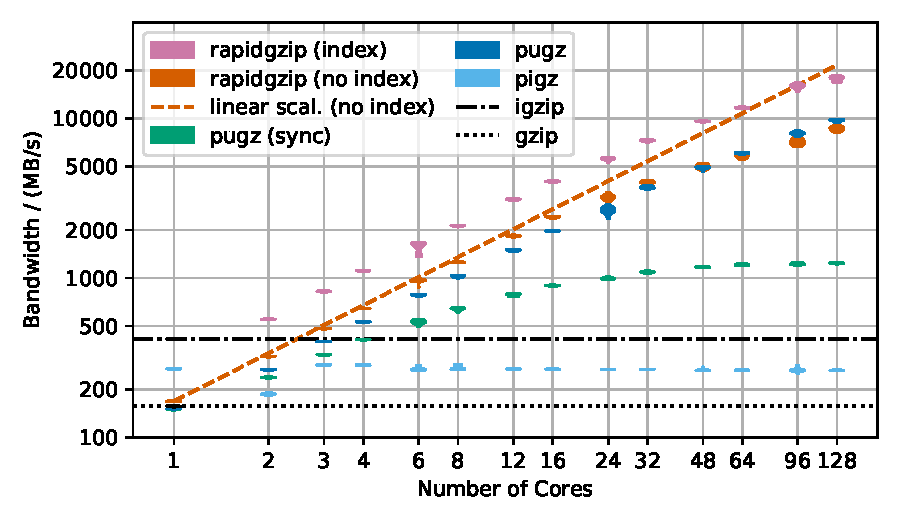
\includegraphics[width=\linewidth]{plots/result-parallel-decompression-base64-dev-null-bandwidths-number-of-threads.pdf}
    \caption{
        Benchmark results for gzip decompression.
        The results are written to \texttt{/dev/null} to avoid I/O write bottlenecks.
        It also makes the benchmarks comparable to those by \citeauthor{pugz}~\cite{pugz}.
        The degree of parallelism is enforced with the respective \texttt{-P} argument for \pragzip and \texttt{-t} for \pugz.
        Furthermore, the command line tool \texttt{taskset} is used to pin the process to a subset of the available cores.
        The file size for the base64 data was chosen to be \SI{128}{\mebi\byte} per core for \texttt{pugz (sync)},
          \SI{512}{\mebi\byte} per core for all other benchmarks of \pragzip and \pugz,
          and \SI{1}{\gibi\byte} for the \CLITOOL{gzip}, \CLITOOL{igzip}, and \pigz benchmarks.
        The violin plot displays the sampled results from repeating the benchmarks 20 times.
    }
    \label{fig:parallel-decompression}
\end{figure}


\cref{fig:parallel-decompression} shows the scaling behavior for parallel decompression for \pugz and \pragzip using base64-encoded random data compressed with \pigz.
\pigz was used to speed up benchmark setup times but triggered race conditions in \pugz.
Such crashes and deadlocks were reduced by setting the \pigz compression option \texttt{-{}-blocksize} to $\SI{4}{\mebi\byte}$ per degree of parallelization.
This option adjusts the workload assigned to each compression thread.
It does not adjust the \deflateblock size, which is \SI{75}{\kilo\byte} of compressed data on average.
Setting this option presumably reduces crashes because it reduces the number of empty \deflateblocks that are used to byte-align the \deflate streams that have been independently compressed by each thread.

\paragraph{Discussion of the Base64-Encoded Random Test Data}
The resulting file has a uniform data compression ratio of \num{1.315} and contains only a few backward pointers.
The compression ratio is mostly achieved with the Huffman coding.
The uniform compression ratio minimizes work distribution effects.
The low frequency of backward pointers makes it possible to fully resolve the markers in a \backrefwindow after a dozen kilobytes of data.
This enables the decoder to replace the two-stage method with single-stage decompression after a while.
The custom \deflate decoder is still used but further optimizations might delegate decompression to zlib in this case.
Therefore, this test data acts as a benchmark for all components except marker replacement.

\paragraph{\Pragzip Performance and Influence of the Index}
\Cref{fig:parallel-decompression} displays the benchmark results for \pragzip.
The benchmark is split into first-time decompression and decompression with an existing index file.
Decompression with an index file is generally faster because of these reasons:
\begin{itemize}
    \item marker replacement can be skipped
    \item the twice as large intermediate 16-bit format can be skipped
    \item decompression can be delegated to zlib
    \item the output buffer can be allocated beforehand in a single allocation because the decompressed size is known
    \item the workload is balanced because chunks in the index are chosen such that the decompressed chunk sizes are similar
\end{itemize}
For this case, \pragzip is the fastest when using more than one thread.
Using \num{128} cores, \pragzip reaches \SI{8.7}{\giga\byte/\second} without an index and \SI{17.8}{\giga\byte/\second} with an index.

\paragraph{Comparing \Pragzip with Pugz}

The bandwidth of \pragzip without a preexisting index is higher than \pugz for fewer than \num{64} cores.
Decompression with \pragzip is assumed to be slower for \num{64} cores and more because it returns the results in the correct order.
This behavior is the same as \texttt{pugz (sync)}, which is slower than \pragzip in all cases.
For this synchronized write mode, \pugz does not scale to more than 32 cores.
It achieves \SI{1.2}{\giga\byte/\second} decompression bandwidth for 48--128 cores.
For \num{128} cores, \pragzip without an index is $7\times$ faster than \texttt{pugz (sync)}.
The unsynchronized version of \pugz writes the decompressed data to the output file in undefined order.
This version has been benchmarked to reproduce the results in the work by \citeauthor{pugz}~\cite{pugz}.
The unsynchronized \pugz and \pragzip do scale to 128 cores but the parallel efficiency decreases.


\paragraph{Comparing \Pragzip with Single-Threaded Gzip Decompressors}

Using \num{128} cores, \pragzip achieves \SI{8.7}{\giga\byte/\second}, a speedup of \num{55} over decompression with gzip with \SI{157}{\mega\byte/\second}, and a speedup of \num{21} over \CLITOOL{igzip}, which decompresses with \SI{416}{\mega\byte/\second}.

When using a single thread, \pragzip reaches \SI{169}{\mega\byte/\second} and is slightly faster than \CLITOOL{gzip}.
It is twice as slow as \CLITOOL{igzip} and also slower than \pigz with \SI{270}{\mega\byte/\second}.
\CLITOOL{igzip} is the fastest single-threaded gzip decompressor.
The bandwidth of \pigz decreases for two cores and then increases again.
Pigz never outperforms \CLITOOL{igzip}.
It is not able to parallelize decompression but it offloads reading, writing, and checksum computation into separate threads.



\subsection{Parallel Decompression of the Silesia Corpus}

\begin{figure}
    \centering
    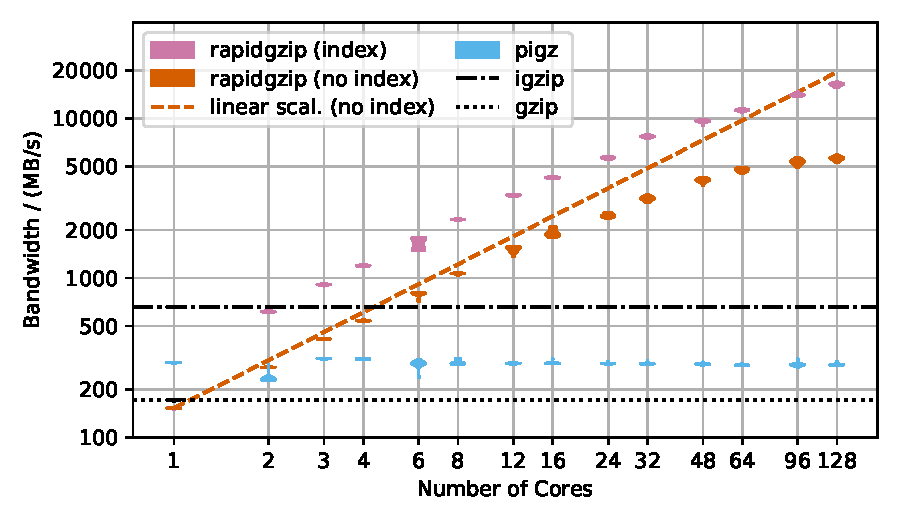
\includegraphics[width=\linewidth]{plots/result-parallel-decompression-silesia-dev-null-bandwidths-number-of-threads.pdf}
    \caption{
        Benchmark results for gzip decompression of a compressed tarball of the Silesia dataset.
        The benchmark setup is the same as for \cref{fig:parallel-decompression}.
        The file size was scaled by concatenating 2 tarballs of Silesia per core.
        Compressing it with \pigz yields \SI{126}{\mega\byte} of compressed data per core.
        This is \SI{424}{\mega\byte} of uncompressed data per core with an average compression ratio of \num{3.1}.
    }
    \label{fig:parallel-decompression-silesia}
\end{figure}

The Silesia corpus~\cite{silesia} is commonly used to benchmark file compression.
\Cref{fig:parallel-decompression-silesia} contains benchmark results for parallel decompression using a gzip-compressed tarball of the Silesia corpus.
The Silesia tarball was concatenated repeatedly to itself to scale the file size with the degree of parallelism.
The comparison does not include \pugz because it is not able to decompress data containing bytes outside of the permitted range of 9--126.
It quits and returns an error when trying to do so.

\pragzip with an index reaches \SI{16.3}{\giga\byte/\second} and \SI{5.6}{\giga\byte/\second} without an index.
Compared to GNU gzip, which reaches \SI{172}{\giga\byte/\second}, this is a speedup of \num{95} and \num{33} respectively.
In comparison to \cref{fig:parallel-decompression}, it stops scaling after $\approx 64$ cores.
This is because the Silesia corpus contains more duplicate strings than base64-encoded random data.
The duplicate strings are compressed as backward pointers, which will be decompressed to markers in the first stage of decompression.
If there are no markers after \SI{32}{\kibi\byte}, the two-stage decompression can fall back to single-stage decompression.
This is the case for base64-encoded random data but not so for the Silesia corpus.
Between the two parallelized stages, the work distributor must resolve the markers in the last \SI{32}{\kibi\byte} of each chunk sequentially.
This limits efficient parallelization according to Amdahl's law.
Increasing the chunk size can alleviate this theoretically but will also increase the cache pressure.

The single-threaded decompression tools in \cref{fig:parallel-decompression-silesia} are faster than in \cref{fig:parallel-decompression} because the backward pointers generate decompressed data faster than undoing the expensive Huffman coding.
In the best case, such a backward pointer can copy 255 bytes from the window to generate a part of the decompressed stream.


\subsection{Parallel Decompression of FASTQ Files}

\begin{figure}
    \centering
    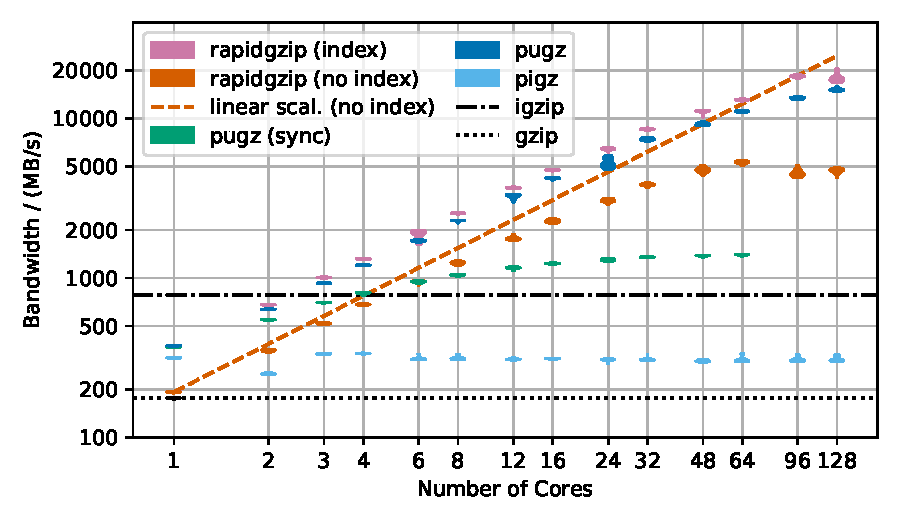
\includegraphics[width=\linewidth]{plots/result-parallel-decompression-fastq-dev-null-bandwidths-number-of-threads.pdf}
    \caption{
        Benchmark results for gzip decompression of a compressed FASTQ file.
        The benchmark setup is the same as for \cref{fig:parallel-decompression}.
        The file size was scaled by concatenating two uncompressed FASTQ files per core.
        Compressing it with \pigz yields \SI{97}{\mega\byte} of compressed data per core.
        This is \SI{362}{\mega\byte} of uncompressed data per core with an average compression ratio of \num{3.74}.
    }
    \label{fig:parallel-decompression-fastq}
\end{figure}

\Cref{fig:parallel-decompression-fastq} contains benchmark results for parallel decompression on a FASTQ file\footnote{        \url{http://ftp.sra.ebi.ac.uk/vol1/fastq/SRR224/085/SRR22403185/SRR22403185_2.fastq.gz}}.
FASTQ files are used for storing biological sequences and metadata.
They were chosen for the benchmark because \pugz was developed to work with them.

Both, \pragzip with an existing index and \pugz without output synchronization scale up to 128 cores while \pragzip is slightly faster in all cases.
Without an index, \pragzip scales up to \num{48} cores and then stops scaling at \SI{4.9}{\giga\byte/\second} peak decompression bandwidth while \pugz with output synchronization scales up to 16 cores reaching a peak decompression bandwidth of \SI{1.4}{\giga\byte/\second}.
Benchmark results for \pugz with synchronization for \num{96} and \num{128} cores are missing because \pugz reproducibly threw errors when decompressing the test file with that many threads.
Overall, the scaling behavior shown in \cref{fig:parallel-decompression-fastq} is similar to that shown in \cref{fig:parallel-decompression-silesia} with the notable exception that \pragzip without an index stops scaling for more than \num{48} cores.


\subsection{Influence of the Chunk Size}

The chunk size, i.e., the amount of compressed data in a work package submitted to the thread pool is one of the parameters that can be optimized.
\Cref{fig:chunk-size} shows that a very small chunk size leads to performance degradation because the overhead caused by the \blockfinder becomes too large.
A very large chunk size leads to performance loss because the work is not evenly distributed to the worker threads.
For \SI{512}{\mebi\byte} and more, the performance for \pugz stays stable because the maximum chunk size is limited to support even work distribution.
In these cases, each thread works on one chunk with a size of \SI{389}{\mebi\byte}.
This is not the case for \pragzip and performance degrades even more because not all worker threads have chunks to work on.
Assertion errors were observed with \pugz for chunks sized \SI{16}{\mebi\byte} and chunk sizes smaller than \SI{8}{\mebi\byte}.
The optimal chunk size for \pragzip is \SI{4}{\mebi\byte} and \SI{32}{\mebi\byte} for \pugz.
This is $8\times$ lower than \pugz owing to the optimized \blockfinder.
A lower chunk size reduces memory consumption.

\begin{figure}
    \centering
    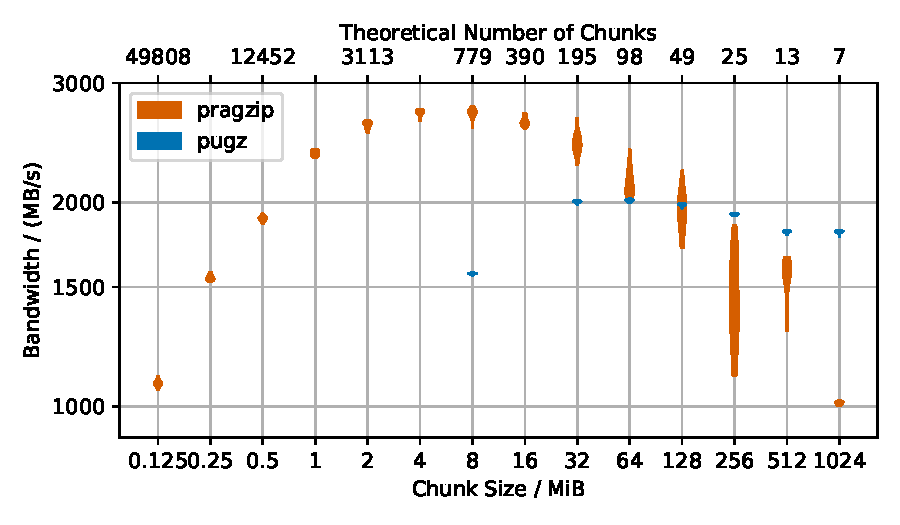
\includegraphics[width=\linewidth]{plots/decompression-chunk-size-bandwidths-number-of-threads.pdf}
    \caption{
        Benchmark results for gzip decompression unhindered by I/O write speeds using \num{16} cores and \SI{8}{\gibi\byte} of base64-encoded random data resulting in a gzip-compressed file size of \SI{6.08}{\gibi\byte}.
        The violin plot displays the sampled results from repeating the benchmarks 20 times.
    }
    \label{fig:chunk-size}
\end{figure}



\subsection{Influence of the Compressor}
\label{sct:gzip-compressors}


\begin{table}
    \centering
    \begin{tabular}{l|S[table-format=1.2]|S[separate-uncertainty, table-format=2.4(4)]}
        Compressor & {Compr. Ratio} & {Bandwidth / (\SI{}{\giga\byte/\second})}\\
        \hline & & \\[-1em]
        bgzip -l -1 & 2.99 &  5.65   +- 0.15   \\
        bgzip -l 0  & 1.00 & 10.6    +- 0.4    \\
        bgzip -l 3  & 2.81 &  5.90   +- 0.21   \\
        bgzip -l 6  & 2.99 &  5.67   +- 0.17   \\
        bgzip -l 9  & 3.01 &  5.64   +- 0.17   \\
        \hline & & \\[-1em]
        gzip -1     & 2.74 &  6.05   +- 0.15   \\
        gzip -3     & 2.90 &  5.55   +- 0.20   \\
        gzip -6     & 3.11 &  5.17   +- 0.15   \\
        gzip -9     & 3.13 &  5.03   +- 0.16   \\
        \hline & & \\[-1em]
        igzip -0    & 2.42 &  0.1586 +- 0.0013 \\
        igzip -1    & 2.71 &  6.15   +- 0.19   \\
        igzip -2    & 2.77 &  6.42   +- 0.14   \\
        igzip -3    & 2.82 &  6.52   +- 0.20   \\
        \hline & & \\[-1em]
        pigz -1     & 2.75 &  3.82   +- 0.07   \\
        pigz -3     & 2.91 &  3.81   +- 0.07   \\
        pigz -6     & 3.11 &  3.76   +- 0.09   \\
        pigz -9     & 3.13 &  3.73   +- 0.07   \\
    \end{tabular}
    \caption{
        The decompression bandwidths for decompressing Silesia with \pragzip using 128 cores.
        The benchmarks were repeated 20 times.
        Uncertainties are given with one standard deviation.
        The Silesia dataset was compressed with a variety of compression tools and compression levels as indicated in the first column.
        The Silesia dataset size was increased by concatenating 256 tarballs of the Silesia dataset.
        This creates a test file totaling \SI{54.2}{\giga\byte}.
    }
    \label{tab:compressors}
\end{table}

We have shown the weak-scaling behavior using \pigz with default compression levels to compress the data in the previous sections.
\Cref{tab:compressors} shows that \pragzip achieves efficient parallel decompression on the Silesia dataset for a wide variety of compression tools and compression levels.
This means that it can be used for almost any gzip-compressed data making it useful for cases in which the compression options cannot be adjusted.

\Cref{tab:compressors} also shows that there is significant variability across different compressors, e.g., decompression of \pigz-compressed files is slower than for \texttt{gzip}-compressed files.
One cause is the average \dynblock size, which can be chosen arbitrarily by the compressor.
There is only one Huffman coding per \dynblock.
The overhead required for reading and preprocessing that Huffman coding can be amortized better for longer \dynblocks.
Conversely, larger \dynblocks result in increased overhead for \pragzip to find the first \deflate block inside a chunk.

The dataset compressed with \texttt{bgzip -0} can be decompressed the fastest because, in this case, \texttt{bgzip} skips compression altogether and stores the data as \rawblocks.
Thus, \pragzip can fall back to a fast memory copy of the \deflate block contents.

The dataset created with \texttt{igzip -0} contains all the compressed data in a single \dynblock.
Therefore, the \pragzip decompression threads cannot find any other \deflate block boundary to start decompression from.
In this case, parallel decompression is not possible and the resulting decompression bandwidth is effectively a single-core decompression bandwidth.

\subsection{Comparison With Other Compression Formats}
\label{sct:compression-formats}

\begin{table}
    \centering
    \begin{tabular}{l|c|l|S[table-format=3]|S[separate-uncertainty, table-format=1.5(5), group-separator={}]}
        Com. & Rat. & Decompressor & {P} & {Bandw. / (\SI{}{\giga\byte/\second})}\\
        \hline & & & \\[-1em]
        bzip2 & 3.88 & lbzip2             & 1   &  0.04492 +- 0.00012 \\
        bgzip & 2.99 & bgzip              & 1   &  0.2977  +- 0.0023  \\
        gzip  & 3.11 & bgzip              & 1   &  0.2965  +- 0.0010  \\
        gzip  & 3.11 & rapidgzip          & 1   &  0.1527  +- 0.0010  \\
        gzip  & 3.11 & rapidgzip (index)  & 1   &  0.1528  +- 0.0007  \\
        gzip  & 3.11 & igzip              & 1   &  0.656   +- 0.009   \\
        zstd  & 3.18 & zstd               & 1   &  0.820   +- 0.006   \\
        zstd  & 3.18 & pzstd              & 1   &  0.816   +- 0.005   \\
        pzstd & 3.17 & pzstd              & 1   &  0.811   +- 0.003   \\
        lz4   & 2.10 & lz4                & 1   &  1.337   +- 0.013   \\
        \hline & & \\[-1em]
        bzip2 & 3.88 & lbzip2             & 16  &  0.667   +- 0.004   \\
        bgzip & 2.99 & bgzip              & 16  &  2.82    +- 0.07    \\
        gzip  & 3.11 & bgzip              & 16  &  0.3017  +- 0.0007  \\
        gzip  & 3.11 & rapidgzip          & 16  &  1.86    +- 0.12    \\
        gzip  & 3.11 & rapidgzip (index)  & 16  &  4.25    +- 0.03    \\
        pzstd & 3.17 & pzstd              & 16  &  6.78    +- 0.14    \\
        zstd  & 3.18 & pzstd              & 16  &  0.882   +- 0.006   \\
        \hline & & \\[-1em]
        bgzip & 2.99 & bgzip              & 128 &  5.5     +- 0.5     \\
        bzip2 & 3.88 & lbzip2             & 128 &  4.105   +- 0.024   \\
        gzip  & 3.11 & rapidgzip          & 128 &  5.13    +- 0.13    \\
        gzip  & 3.11 & rapidgzip (index)  & 128 & 16.43    +- 0.27    \\
        pzstd & 3.17 & pzstd              & 128 &  8.8     +- 0.8     \\
        pzstd & 3.17 & pzstd (no check)   & 128 &  8.8     +- 0.6     \\
    \end{tabular}
    \caption{
        The decompression bandwidths for a variety of decompression tools executed with fixed parallelization P.
        Uncertainties are given with one standard deviation.
        The first column shows the tool used for creating the compressed file when using default compression levels.
        The second column shows the compression ratio of the file.
        The file size was scaled by concatenating 2 tarballs of Silesia per core.
        This fixes the uncompressed file sizes to \SI{424}{\mega\byte}, \SI{3.39}{\giga\byte}, and \SI{27.13}{\giga\byte} for a parallelization of \num{1}, \num{16}, and \num{128} respectively.
    }
    \label{tab:compression-formats}
\end{table}

\begin{table}
    \centering
    \begin{tabular}{l|l||l|l}
        Software & Version & Software & Version \\
        \hline & & & \\[-1em]
        bgzip     & 1.17     &   pigz      & 2.7      \\
        gzip      & 1.12     &   pugz      & cc7c9942 \\
        igzip     & 9f2b68f0 &   pzstd     & 1.5.4    \\
        lbzip2    & 2.5      &   rapidgzip & d4aa8d4b \\
        lz4       & 1.9.4    &   zstd      & 1.5.4    \\
    \end{tabular}
    \caption{
        Software versions or git commit hashes used for benchmarks.
    }
    \label{tab:software-versions}
\end{table}

To conclude the benchmark section, we provide benchmark results for other compression formats in \cref{tab:compression-formats}.
Only default compression levels were included.
For a more comprehensive comparison of compression formats benchmarked with one core, we refer to lzbench~\cite{lzbench}.
Multiple things are of note in \Cref{tab:compression-formats}.

As can be seen for parallelization on 16 cores, both, \bgzip and \pzstd require specially prepared gzip and zstd files, respectively, to achieve parallelized decompression.
For \pzstd, Zstandard files with more than one frame are required but \CLITOOL{zstd} creates only Zstandard-compressed files with a single frame.
\Pragzip and \CLITOOL{lbzip2}~\cite{lbzip2} can work with arbitrary gzip and bzip2 files respectively.

Single-threaded \pragzip achieves \qty{153}{\mega\byte} decompression bandwidth while \bgzip is $\num{1.9}\times$ as fast and \CLITOOL{igzip} even $\num{4.3}\times$ as fast.
This shows further optimization potential for the custom-written \deflate implementation in \pragzip.

\CLITOOL{zstd} and \CLITOOL{pzstd} are $\num{5.4}\times$ faster than the single-core \pragzip but only $\num{1.2}\times$ faster than \CLITOOL{igzip} .
However, \CLITOOL{pzstd} cannot effectively use many cores.
The achieved speedup when using \num{16} cores instead of one core is \num{8.4}.
For \num{128} cores, the achieved speedup is \num{10.9}.
This ineffective parallelization closes the gap between \pragzip and \CLITOOL{pzstd} for larger core counts.
For 128 cores, \pragzip with an existing index becomes twice as fast as \CLITOOL{pzstd}.

The command line tool \CLITOOL{lbzip2} can be used for parallelized bzip2 decompression.
While \pzstd is $\num{18}\times$ faster than \CLITOOL{lbzip2} when using one core, it only is $\num{2.1}\times$ faster when using \num{128} cores.
Disabling checksum computation in \pzstd using the \texttt{-{}-no-check} option did not improve the decompression bandwidth.

The limited parallel scaling of \pzstd shows performance potential for the parallel architecture.
Alternatively, parallel Zstandard decompression could be implemented in the \pragzip architecture shown in \cref{fig:architecture} as has already been done for bzip2.
